\chapter{序論}
\label{chap:introduction}

本章では、本研究の動機と目的、および本論文の構成について述べる。

\newpage

\section{研究の動機}

ワイヤレスネットワークや小型計算機の普及によるIoT社会が到来しつつある現在,
人々は時刻、メール、SNS、天気予報、ニュースなどの大量のリアルタイム情報や通知メッセージなどに圧倒されている.
これらの情報の表示には投稿を時系列に並べる{\bf タイムライン表示}(図\ref{timeline})を用いることが現在の主流であるが、
多くの情報を人間が理解しやすくするため,以下のような視覚化手法も利用されている.

\begin{figure}[H]
\centering
\fbox{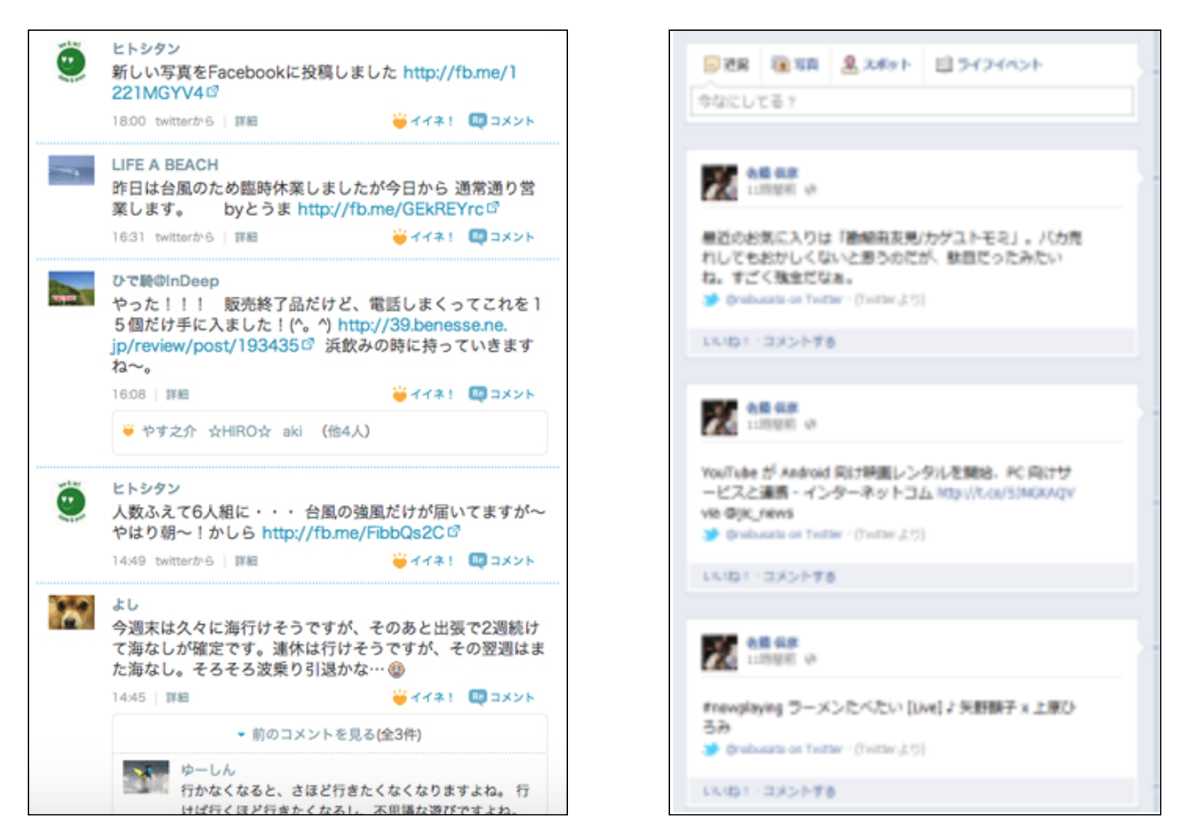
\includegraphics[width=9cm]{images/timeline.png}}
\caption{タイムライン表示}
\label{timeline}
\end{figure}

\vspace{3mm}

\paragraph*{情報ダッシュボード}

情報ダッシュボード\cite{few}は,
複数のリアルタイム情報をタイル状に並べて表示することによって
多くの情報をわかりやすく視覚化するシステムである.
たとえばWindowsのスタート画面(図\ref{windows})の情報ダッシュボードには
天気予報や株価のようなリアルタイム情報を表示可能である.

\begin{figure}[H]
\centering
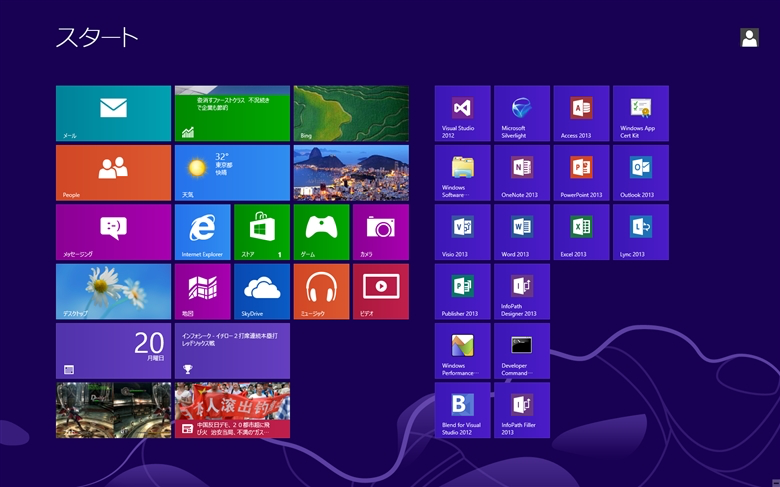
\includegraphics[width=9cm]{images/windows.png}
\caption{Windowsのスタート画面}
\label{windows}
\end{figure}

\vspace{2mm}
\paragraph*{スタンプ}

リアルタイムに流れていくタイムライン表示の中で情報を目立たせたいとき,
近年「スタンプ」と呼ばれるピクトグラムが
利用されることが多くなってきた(図\ref{linestamp}).

スタンプはテキストで記述するのが難しい表現や感情を伝えたり,
テキストを考えて入力するよりも速くて簡単であったりすることから,
近年LINEやFacebookメッセンジャー,オンラインゲームなどで広く利用されている.

\begin{figure}[H]
\centering
\fbox{
\includegraphics[width=5cm]{images/linestamp.png}}
\caption{LINEのスタンプの例}
\label{linestamp}
\end{figure}

\section{本研究の目的}
「情報ダッシュボード」の利用は広まっているが,利用できる情報の種類は限られており,
ユーザが情報を投稿して共有することはできない.
スタンプ的な表現を投稿可能な情報ダッシュボードを用意し,
その上でネット上の情報やユーザの感情/気分などを表示すれば,
現在の世界や人々の状況を一目了然に理解する(わかる)ことが可能になるであろう.
実世界の状態や人間の状況を情報ダッシュボードにわかりやすく表示し,
かつ誰もが簡単に気分などをスタンプのように投稿して共有できるシステムを開発することを目的とする.

\section{本論文の構成}

本論文は以下の8章で構成される。

第2章では、本研究の背景をより詳細に分析し、既存の視覚化システムの問題点を整理する。

第3章では、関連する研究分野についてまとめ、それぞれの利点と問題点を整理する。

第4章では、本論文で提案する視覚化システムの概要と全体像を示し、
システム全体の構成と実現すべきユーザ体験について述べる。

第5章では、本論文で提案するシステムの具体的な実装について述べる。

第6章では、本論文で提案するシステムの評価実験の概要と結果を述べる。

第7章では、第6章での結果を考察し、本論文で提案するシステムの有効性と意義について議論を行う。

最後に、第8章で本論文のまとめと結論を述べる。